%%%%%%%%%%%%%%%%%%%%%%%%%%%%% Define Article %%%%%%%%%%%%%%%%%%%%%%%%%%%%%%%%%%
\documentclass{article}
%%%%%%%%%%%%%%%%%%%%%%%%%%%%%%%%%%%%%%%%%%%%%%%%%%%%%%%%%%%%%%%%%%%%%%%%%%%%%%%
%%%%%%%%%%%%%%%%%%%%%%%%%%%%% Using Packages %%%%%%%%%%%%%%%%%%%%%%%%%%%%%%%%%%
\usepackage{geometry}
\usepackage{graphicx}
\usepackage{amssymb}
\usepackage{amsmath}
\usepackage{amsthm}
\usepackage{empheq}
\usepackage{mdframed}
\usepackage{booktabs}
\usepackage{lipsum}
\usepackage{graphicx}
\usepackage{color}
\usepackage{psfrag}
\usepackage{pgfplots}
\usepackage{bm}
%%%%%%%%%%%%%%%%%%%%%%%%%%%%%%%%%%%%%%%%%%%%%%%%%%%%%%%%%%%%%%%%%%%%%%%%%%%%%%%

% Other Settings

%%%%%%%%%%%%%%%%%%%%%%%%%% Page Setting %%%%%%%%%%%%%%%%%%%%%%%%%%%%%%%%%%%%%%%
\geometry{a4paper}

%%%%%%%%%%%%%%%%%%%%%%%%%% Define some useful colors %%%%%%%%%%%%%%%%%%%%%%%%%%
\definecolor{ocre}{RGB}{243,102,25}
\definecolor{mygray}{RGB}{243,243,244}
\definecolor{deepGreen}{RGB}{26,111,0}
\definecolor{shallowGreen}{RGB}{235,255,255}
\definecolor{deepBlue}{RGB}{61,124,222}
\definecolor{shallowBlue}{RGB}{235,249,255}
%%%%%%%%%%%%%%%%%%%%%%%%%%%%%%%%%%%%%%%%%%%%%%%%%%%%%%%%%%%%%%%%%%%%%%%%%%%%%%%

%%%%%%%%%%%%%%%%%%%%%%%%%% Define an orangebox command %%%%%%%%%%%%%%%%%%%%%%%%
\newcommand\orangebox[1]{\fcolorbox{ocre}{mygray}{\hspace{1em}#1\hspace{1em}}}
%%%%%%%%%%%%%%%%%%%%%%%%%%%%%%%%%%%%%%%%%%%%%%%%%%%%%%%%%%%%%%%%%%%%%%%%%%%%%%%

%%%%%%%%%%%%%%%%%%%%%%%%%%%% English Environments %%%%%%%%%%%%%%%%%%%%%%%%%%%%%
\newtheoremstyle{mytheoremstyle}{3pt}{3pt}{\normalfont}{0cm}{\rmfamily\bfseries}{}{1em}{{\color{black}\thmname{#1}~\thmnumber{#2}}\thmnote{,--,#3}}
\newtheoremstyle{myproblemstyle}{3pt}{3pt}{\normalfont}{0cm}{\rmfamily\bfseries}{}{1em}{{\color{black}\thmname{#1}~\thmnumber{#2}}\thmnote{,--,#3}}
\theoremstyle{mytheoremstyle}
\newmdtheoremenv[linewidth=1pt,backgroundcolor=shallowGreen,linecolor=deepGreen,leftmargin=0pt,innerleftmargin=20pt,innerrightmargin=20pt,]{theorem}{Theorem}[section]

\theoremstyle{mytheoremstyle}
\newmdtheoremenv[linewidth=1pt,backgroundcolor=shallowBlue,linecolor=deepBlue,leftmargin=0pt,innerleftmargin=20pt,innerrightmargin=20pt,]{definition}{Definition}[section]
\theoremstyle{myproblemstyle}
\newmdtheoremenv[linecolor=black,leftmargin=0pt,innerleftmargin=10pt,innerrightmargin=10pt,]{problem}{Problem}[section]


%%%%%%%%%%%%%%%%%%%%%%%%%%%%%%%%%%%%%%%%%%%%%%%%%%%%%%%%%%%%%%%%%%%%%%%%%%%%%%%

%%%%%%%%%%%%%%%%%%%%%%%%%%%%%%% Plotting Settings %%%%%%%%%%%%%%%%%%%%%%%%%%%%%
\usepgfplotslibrary{colorbrewer}
\pgfplotsset{width=8cm,compat=1.9}
%%%%%%%%%%%%%%%%%%%%%%%%%%%%%%%%%%%%%%%%%%%%%%%%%%%%%%%%%%%%%%%%%%%%%%%%%%%%%%%
\begin{document}




\title{
	AI Notes

}
\author{
	Viv Sedov --- \texttt{viv.sedov@hotmail.com}
}
\maketitle

\tableofcontents

\newpage



\section{Propositional\_logic}

\subsection{Simple Operations}
When covering this : there are simple operations that you should know about :

Simple Operation Not:

\[\begin{array}{c | c}
		p & \neg p \\
		\hline
		1 & 0      \\
		0 & 1
	\end{array}
\]

Such that in this case it is the opposite given value $\neg p $ would be the direct opposite of the given Value of P .

For example say that you have the following

\[\begin{array}{c c | c}
		p & q & p \land q \\
		\hline
		1 & 1 & 1         \\
		1 & 0 & 0         \\
		0 & 1 & 0         \\
		0 & 0 & 0
	\end{array}\]
In this example, we are stating the following command : $\neg(14 > 6)$ is false , we create this truth table to prove if that is true or not .

$P \land Q $ is true $\iff$ p and q are true

Simple $\lor$ - OR


\[\begin{array}{c c | c}
		p & q & p \lor q \\
		\hline
		1 & 1 & 1        \\
		1 & 0 & 1        \\
		0 & 1 & 1        \\
		0 & 0 & 0        \\
	\end{array}\]

In this example above , for this to hold true, atleast one of the values would have to have a one it to hold true, this is known as an \textit{Inclusive} or as in you can say the following and it would make sense:
\textbf{I will go to the shops $\lor$ i will go to the coast}\\

\\

Simple Operation $\implies$
This is where if something is true the other must be true , or where you given an equivalent pointer to if p then q


\[\begin{array}{ c c | c }
		p & q & p \implies q \\
		\hline
		1 & 1 & 1            \\
		1 & 0 & 0            \\
		0 & 1 & 1            \\
		1 & 1 & 1            \\
	\end{array}\]


With the above example this is not cause and effect , there is a reason for why this occours , and that is that there is a pointer such that it acts like an if statment, with the following code shown below :

\begin{lstlisting}
foo = True
if foo:
    return 1
else:
    return 0
\end{lstlisting}

The code above is rather simple , but shows that if something is true , then you would have some sort of value expression , or some pointer that would return if it is correct or not .

In the weird scenario of f and t , where if f is false it implies that q is true , that is because  the q value is true , meaning that it would hold , a little trick for this one is that for what ever the second value is , if it is true , it will hold , if both are false , then it will true , though if one is true and the other is false , it will not hold .\\

Logically equivalent $\iff$ this can also be seen as if and only if or iff \\
Here is an example of the logical truth table behind this
\[\begin{array}{c c | c }
		p & q & p \iff q \\
		\hline
		1 & 1 & 1        \\
		1 & 0 & 0        \\
		0 & 1 & 0        \\
		0 & 0 & 1        \\
	\end{array}\]

With this , Where if something is true then the other must be true or if its false then the other would have to be false , in this case you are seeing if these two values are the same .

Example Exersises of how this would all work :
\\
Given that :
\[p = Logic is fun for jane \\ \\
	q = david does not like cabbage \\ \\
	r = david eyes are blue \]\\

We can then further express all of this in a notational form .
\begin{itemize}
	\item $\neg p \land q$
	      This would imply the following truth table
	      \[\begin{array}{c c c | c }
			      \neg p & p & q & \neg p \land q \\
			      \hline
			      0      & 1 & 1 & 0              \\
			      1      & 0 & 1 & 1              \\
			      0      & 1 & 0 & 0              \\
			      1      & 0 & 0 & 0
		      \end{array}\]
	\item $\neg R \land \neg P \implies$  Both are not goint to be true such that you would get only one possible answer for this  .
\end{itemize}


Multiple truth table example :
show the following in a truth table :
\\
\[p \land (q \implies r) \]

\[\begin{array}{c c c | c | c }
		p & q & r & q \implies r & p \land (q \implies r) \\
		\hline
		1 & 1 & 1 & 1            & 1                      \\
		1 & 1 & 0 & 0            & 0                      \\
		1 & 0 & 1 & 1            & 1                      \\
		0 & 1 & 0 & 0            & 0                      \\
		0 & 1 & 1 & 1            & 0                      \\
		0 & 0 & 0 & 1            & 0                      \\
	\end{array}\]

Here is another example to understand how these tables would all work together
\\
\[(p \implies q) \land (q \implies p)\]
\[\begin{array}{c c c | c | c}
		p & q & q \implies p & p \implies q & (p \implies q) \land (q \implies p) \\
		\hline
		1 & 1 & 1            & 1            & 1                                   \\
		0 & 1 & 0            & 1            & 0                                   \\
		1 & 0 & 1            & 0            & 1                                   \\
		0 & 0 & 1            & 1            & 1                                   \\
	\end{array}\] \\

\\ \\


\begin{definition}
	Two propositions are equal if they have the same truth values , they are known as $ P \implies Q$ this is known as logically equivalent
\end{definition}

\begin{definition}
	A proposition is tautology if it is always true an example of this is $ P \lor \neg P$ this is always true

\end{definition}

\begin{definition}
	A proposition is a contradiction if it is always false for example $ P \land \neg P $ this is always false
\end{definition}

\begin{definition}
	A proposition is \textbf{Contingent} if it is neither Always true or false
\end{definition}

\\
\section{Disjunctive Normal Form}
A given formula is said to be a \textit{Disjunctive normal form} when it is an Or $\implies \lor$ this is known as \textbf{DNF} a function is conjunctive when it has an $ \land $ form , within their proposition logic .

\[(p \land \neg q \land r) \lor (\neg q \land \neg r) \lor q \]

Everytime a given formula is built , we would folow the rules of propositional calculus , and how for each conjunctive formula there should be a disjunctive formula as well .

\subsection{DNF of mini terms for truth tables}
\begin{itemize}
	\item For each row whose truth value is true , write doen for each of the prposition variables , of $ p_i $ in the formula of it self , either $P_i$ is true in row or $\neg P_i$ if false.
	\item Repeate the first pointer , for the truth table where the formula is true and write down the dijunction of the conjuctions .
\end{itemize}

What you will rsee is that those two values will equal up such that the result of the formula in DNF is the equivalent to the original formula .

\section{Conjunctive Normal Form}
A formula is said to be \textbf{Conjunctive Normal Form} when its conjunction is $ \land $ of disjunctive of $ \lor $ an example of this is shown below :
\[(\neg P \lor Q \lor R \lor \neg S) \land (P \lor Q) \land \neg S \land (Q \lor \neg R \lor S)\]

Every expression built up according to the rules of calc , and suchj that for each conjunctive formula there is a similar or an equivelent formual that can be written in disjunctive form .

\paragraph{Summary}
\item Conjunctive form , or in brackets , and on the outside
\item Disjunctive form,  And in the brackets and or on the outside
\newpage
\section{Logical Equivalences}
We can use this to obtain normal form , when we use the implication law to eliminate subproccess - when ever you have a doubel negation and demorgans to bring a $ \neg $ you what this value to be on the outside  : here are the sub process of how this can be done :


\[\neg\neg P \iff P \]
This rule is the double negation Law \\ \\

\[ \begin{array}{c}
		(P \lor Q) \iff (Q \lor P)   \\
		(P \land Q) \iff (Q \land P) \\
		(P \iff Q) \iff (Q \iff P)
	\end{array}\]
Commutaive laws where both values would have to equal towards each other  .


\[\begin{array}{c}
		((P \lor Q) \lor R) \iff (P \lor (Q \lor R))    \\
		((P \land Q) \land R) \iff (P \land(Q \land R)) \\
	\end{array}\]
This is the associative laws , where it is very similar to how they work in matricies in which they can equate towards each other . \\

\[\begin{array}{c}
		((P \lor Q) \land R) \iff (P \lor (Q \land R)) \\
		((P \land Q) \lor R) \iff (P \land(Q \lor R))  \\
	\end{array}\]
This lase is the distributive law , in which the given values would be changed within a DNF and CNF representation

\[\begin{array}{c}
		(P \lor P) \iff P \\
		(P \land P) \iff P
	\end{array}\]
Idempotent laws where the values of it self would always equal to it self no matter what .

\item Demorgans Law :

\[\begin{array}{c}
		\neg(P \lor Q) \iff (\neg P \land \neg Q) \\
		\neg(P \land Q) \iff (\neg P \lor \neg Q) \\
		(P \land Q) \iff \neg(\neg P \lor \neg Q) \\
		(P \lor Q) \iff \neg(\neg P \land \neg Q) \\
	\end{array}\]
Most times when you lookat demorgans law , you will notice that its very similar to the laws that have been stated above, but the thing that you want to note is that you will see that they are equal in some sense ,  where an or , is a direct link with Not  and And it self.


\item $\S$ Contrapositive Laws
\[\begin{array}{c}
		(P \implies Q) \iff (\neg Q \implies \neg P)
	\end{array} \]

implication that imply towards each other are contrapositive and hence you can switch out the given details of that infomation .

where If Q is an active reciever then P must be an active pointer is the same as stating if not p equates to Not q, in some sense you should understand how that would work .

\item $\S$  Implication
\[\begin{array}{c}
		(P \implies Q) \iff (\neg P \lor Q) \\
		(P \implies Q) \iff \neg(P \land \neg Q)
	\end{array}\]

\item  $\S$ Furhter implication
\[\begin{array}{c}
		(P \lor Q) \iff (\neg P \implies Q) \\
		(P \land Q) \iff \neg(\neg p \implies \neg Q)
	\end{array}\]
Thi sone is rather annyoing , but the principle of how this works is very intriguing , if you do prove this via proof table you will see that they are truly equivalent:
$P \lor Q$

\[\begin{array}{c c | c}
		p & q & p \lor q \\
		\hline
		1 & 1 & 1        \\
		1 & 0 & 1        \\
		0 & 1 & 1        \\
		0 & 0 & 0        \\
	\end{array}\]



this is the same as :
$(\neg P \implies Q) $


\[\begin{array}{c c c | c}
		P & Q & p \implies Q & (\neg P \implies Q) \\
		\hline
		1 & 1 & 1            & 1                   \\
		0 & 1 & 1            & 1                   \\
		1 & 0 & 0            & 1                   \\
		0 & 0 & 1            & 0                   \\
	\end{array}\]

If you look at the given tables above you will notice that indeed they are the same, a truth tabel may be long but they are very good at breaking down the given data that you have into something more readble .


\item Further Implies and equivalences

\[\begin{array}{c}
		((P \implies R) \land (Q \implies R)) \iff ((P \lor Q) \implies R)   \\
		((P \implies Q) \land (P \implies R)) \iff ((P \implies (Q \land R)) \\
	\end{array}\]
With this law you are using the given equivelences that are shown above with the disjunctive and conjunctive views ,but within an equivelence ratio


\item  $\S$ Exportion Law
\[\begin{array}{c}
		((P \land Q) \implies R) \iff (P \implies (Q \implies R))
	\end{array}\]

This one is a good one , Mainly because if anything that does imply to another pointer , you can show that they are all equal towards each other .



\item $\S$ Side Notes
Within the compound proposition $\neg(P \lor Q) \&  (\neg P \land \neg Q) $ they are the same , hence why when you look at the proof that is shown above you will see that they are the same .

When ever you look at equivelences you will notice that connectives $ \lor \land $ will allways suggest that $ P \lor Q \implies Q \lor P $

\newpage

\section{Formal definition }

\begin{definition}[Valid]
	An argument would be considered valid if and only if it takes a form that makes it impossible fro the premise to be true, in the sense that the conclusion is never going to be false. it is not possible to show it to be false in some sense.
	A formula is valid if and only if it is true under every understanding of its given argument, or its given schema, we can say it is valid if true holds for everything..
\end{definition}

\begin{definition}[Sound implies Valid]
	Valid allows us to imply Soundness

	We can say that if you have a valid argument, then you also have a sound statement.
	am argument would be considered sound if it is valid and all the premise is true.
\end{definition}

\begin{definition}
	Sound, in logic a premise or conclusion is said to be valid if it is true under every possible understanding of its given argument, or its given schema.
	\begin{center}
		\begin{tabular}{ c c c }
			1  & 2 & 1 \\
			\hline
			24 & 5 & 1 \\
			\hline
			7  & 8 & 1
		\end{tabular}
	\end{center}

	The example their would be both valid and sound
	\begin{math}
		\forall axiom \exists axiom \implies \vdash A
	\end{math}
	What this just means is that A consist of either an axiom or can get derived from an axiom set using only the rules of inference

	\textbf{\textit{To Dumb this down even more, if you have statement x and you want to prove statement y, you can only do so by breaking x down into smaller statements to see if you can prove and show that y exists}}
	\\
	\begin{math}
		\forall x \exists y \implies \vdash y  \\
		\forall x \exists y \implies \vdash x \land y \\
		\forall x \exists y \implies \vdash x \lor y \\
		\forall x \exists y \implies \vdash x \implies y \\
		\forall x \exists y \implies \vdash x \iff y \\
		\forall x \exists y \implies \vdash x \leftarrow y \\
		\forall x \exists y \implies \vdash x \rightarrow y \\
		\forall x \exists y \implies \vdash x \leftrightarrow y \\
	\end{math}

	Thing to note is that it does \textit{Not} mean that \textbf{A is satisfied} this is a deduction but if you want to show satisfaction you would have to show

	\begin{math}
		A \ \ indicates \ \ \forall Axiom A \\
		\forall A A(\models A) \implies True
	\end{math}

\end{definition}

\begin{theorem}[Validity of statement]
	Validity says nothing about whether or not any statement of the premises is true or not, it only says that the conclusion is true under every possible understanding of the premises.
	the key work their is Understanding of its own premises .

	Such that validity states that its more about the form of an argument than it being true of it self.
\end{theorem}

So we can say a argument is valid if it has the proper form . An argument can have the right form, but be false.
\\
\begin{tt}
	Daffy Duck is a duck \\
	All ducks are insects \\
	their for daffy duck is a insect \\
\end{tt}

Notice how these argument contain a form for \textit{if x is Y} but then you see that they are not true.
Notice However that if the premises \textbf{Were} True then the conclusion would also have to be true - this is a valid proof for validity. A valid argument needs not have true premises or a true conclusion.

\begin{theorem}[Sound requires a true premises]
	Sound logically implies that a statement is true, this is due to the fact that, when a statement is sound, it means that it has a true premises and a true conclusion, we can formally derive x from y using this factor.

	\textbf{\textit{Soundness}} Is an argument or a factor if it means the following arguments

	\begin{itemize}
		\item It is valid
		\item it has a true premises
	\end{itemize}
\end{theorem}

\begin{enumerate}
	\item  Sound requires both valid and to have a true premisies
	\item for all valid arguments if the premises are true then the conlusion must also be true
\end{enumerate}

Example :

\begin{enumerate}
	\item All rabits are mammals
	\item bugs bunny is a rabbit
	\item Therfore, Bugs bunny is a mammal
\end{enumerate}
In this argument we state that all of the premises are true, then the conclusion is true, so it is valid, and the premises are true, all rabbitss in fact are mammals and bugs bunny is a rabitt - so our conclusion makes sense.

\begin{definition}
	Completeness
	\begin{displaymath}
		\alpha \models \beta \implies \alpha \vdash \beta
	\end{displaymath}
	i.e if we can show something is true, then we can say that it is provable - we want to be able to prove all true statements, but you can also get false statements - such that you can prove both false and true Statements, such that if you end up proving false then your statement is no longer sound.
\end{definition}
\newpage

\begin{definition}
	Soundness
	\begin{displaymath}
		\alpha \vdash \beta \implies \alpha \models \beta
	\end{displaymath}
	If we have a formulation i.e xy = 10, then we want to be able to show that fact. We do not want a system where we start out with something true and dedice something to be false, if we know something we should prove with our current knoweldge of breaking something down, that given statement would hold, through infierence rules.

	However it is conceivable that even if our system is sound, it maybe incomplete, regarding what it can express hence why it requires to have a competes property to ensure that our given formulation of our proof would hold true.


\end{definition}


\subsection{Summary without the crap }
If your KB \textit{Knowledge base }Entails Q then all interpretations ( assigning true or false ) values to variables that would allow you to evaluate your knowledge to True, also evaluates to Q to true
\begin{math}
	KB \models Q
\end{math}
\item Entailment refers to how premises lead to a conclusion
reacall how m(b) is a subset of m(a)

\begin{align}

	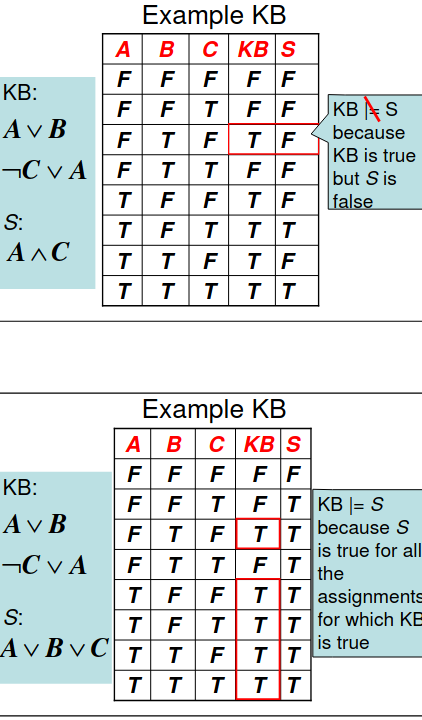
\includegraphics[width=200px]{../img/2022-03-18-16-26-04.png}
\end{align}
Leads into

\begin{align}
	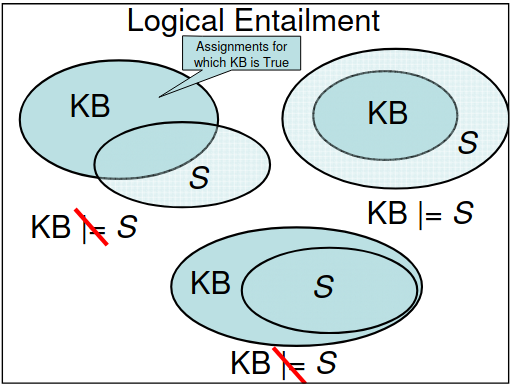
\includegraphics[width=200px]{../img/proofOfModel.png}
\end{align}

Inference is a procedure for deriving a new sentence ‘p’ from ‘KB’ following some algorithm.
\begin{math}
	KB \vdash p
\end{math}
The inference algorithm is sound if it derives only sentences that are entailed by KB. The inference algorithm is complete if whatever can be entailed by KB can also be inferred from KB.
Basically, an inference is an informal and less reliable kind of entailment.

\begin{itemize}
	\item We have a kb
	\item We have some sentence S - query
	\item we want to prove S from our KB
	\item We say it is sound and complete if the space of model is finite within 2 pow n
\end{itemize}

\begin{align*}
	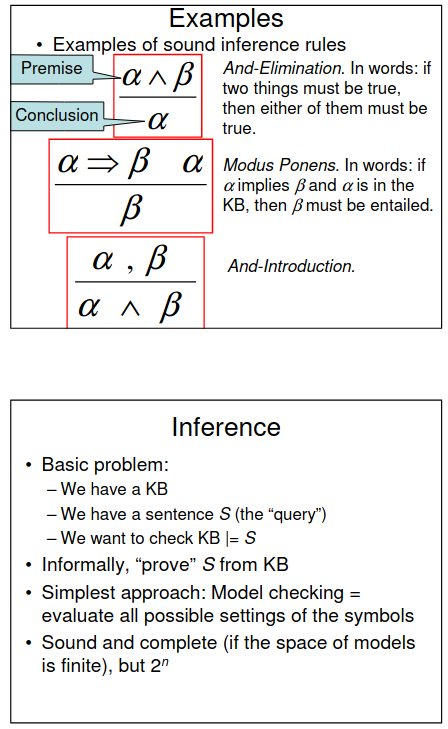
\includegraphics[width=200px]{../img/2022-03-18-16-45-07.png}
\end{align*}

\subsection{Equivalences and normal form }

\begin{definition}
	A sentance is valid if it is true in all models
	\begin{displaymath}
		True, \alpha \lor \neg \alpha , \alpha \implies \alpha , (\alpha \land (\alpha \implies \beta )) \implies \beta
	\end{displaymath}
	We can say that Validity is directctly connected through the inference of the deduction theorum
	\begin{displaymath}
		KB \models \alpha  \iff(KB* \implies \alpha )
	\end{displaymath}
\end{definition}


\section{Resolution algorithm}
\begin{itemize}
	\item input Kb and S
	\item Output true if
	      $KB \models S$ False otherwise
	\item  Initalise a list of clauses  CNF(KB and not S)
	      \begin{itemize}
		      \item for each pair of clauses C i and c h
		      \item R implies resolution of i and j
		      \item new resolution is made
	      \end{itemize}
	\item If clauses are new then return false
	\item if cluauses unifie each other return true
\end{itemize}

\newpage
\subsection{Resolution properties}
\begin{itemize}

	\item Resolution is Sound i.e it produces a sentence that are entailed by their orginal owner
	\item Resolution is complete - it is guarantee to establish entailment of the query for every finite time
	\item Completeness is based on the key theorem
	      \begin{theorem}
		      If a set of clauses is unsatisfiable, then the set of all clauses that can be obtained by the resolution contains an empty clause
	      \end{theorem}
	\item So in short, we can say the opposite of a resolute theorem is that if we cannot find the empty clause the query must be satisfiable.
\end{itemize}

We use resolution to check consistency of how KB holds
\begin{math}
	Human \implies Mortal\\
	Peter \implies Human
\end{math}
We convert that into CNF
\begin{math}
	\neg Human \lor Mortal\\
	\neg Peter \lor Human \\
\end{math}
We can then give our resolution to this being
\begin{math}
	\neg Peter \lor Mortal
\end{math}

\begin{align}
	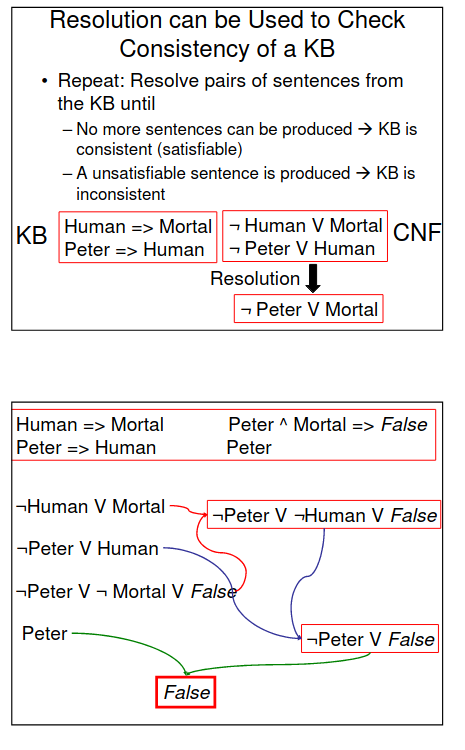
\includegraphics[width=200px]{../img/2022-03-18-17-42-10.png}
\end{align}
Here in this image you can see how we can go from one proof, after another by linking them, to return if a valid argument will be true or false.



\subsection{Horn Form KB}
Horn Form is a clause or a form in which a logical inference problem is given :
Given : \\
\begin{itemize}
	\item A KB is a set of information
	\item A sentance $\alpha \implies theorem $
\end{itemize}

If a sentence is in KB, are restricted to some special form, some of the sound inference rules might be complete . In short its being able to convert from CNF form into implication rules
\\
\begin{math}
	(\alpha \lor \neg \beta) \land (\neg \alpha \lor \neg \gamma \lor \delta ) \\
	\iff \\
	(\beta \implies \alpha ) \land (\alpha \implies \gamma) \implies \delta)
\end{math}
This is known as horn form normal form.

\begin{itemize}
	\item Two inference rules that are sound and complete with respect to properistional symbols for kb in the hron normal form
	      \begin{itemize}
		      \item resolution on a positive unit
		      \item Modus pones
	      \end{itemize}
\end{itemize}

\begin{itemize}
	\item Have to be in conjuctive form \( \lor \ldots \lor  \ldots \lor  \ldots \)
	\item Would Follow the three basic principles
	      \begin{itemize}
		      \item fact
		      \item Goal
		      \item Rule
	      \end{itemize}
	      These are defined whith the following statement
	\item Rule :
	      \begin{math}
		      Man and Gel \implies Tall
	      \end{math}
	      Saying Gel men are tall
	      this can be counter proved with the following statement to prove completness
	      \begin{math}
		      KB \models \alpha \iff(KB* \land \neg \alpha) \text{not provable to be satisfiable i.e unsatisfiable }

	      \end{math}
	      You want to end up showing that thing you are trying to prove may or may not have any models
\end{itemize}
\section{Chaining}
$\implies$ Just look at the slides

\section{Total Summary of propositional logic}
\begin{theorem}
	Inference: process of deriving sentences entailed by the KB
	\begin{displaymath}
		KB \vdash_i \alpha
	\end{displaymath}
	is a sentance where \( \alpha  \) can be derived from KB in teh process of i
\end{theorem}

\textbf{\textit{For first-order logic there exists a sound and complete inference procedure
		- i.e. the procedure will answer any question whose answer follows from
		what is known by the KB.}}

\subsection{Formal Definitions}
\begin{itemize}
	\item \begin{definition}[Syntax]
		      \textit{Syntax}: formal structure of how a sentence is made
	      \end{definition}
	\item \begin{definition}[Semantics]
		      \textit{Symatics}: Truth of sentences with respect of the model
	      \end{definition}
	\item \begin{definition}[Entailment]
		      \( KB \models \alpha \iff true \in \mathbf{T}, \forall Models \ \ KB\)
	      \end{definition}
	\item \begin{definition}[Sound]
		      Derivations produced only from entailed sentances
	      \end{definition}

	\item \begin{definition}[Completeness]
		      Can you prove your derived formulation from - any derivations can produce the same theorm in return
	      \end{definition}
\end{itemize}

\subsection{Syntax}
\begin{itemize}
	\item \begin{definition}[Atomic]
		      \( \perp \) , \(\neg \perp \) Or P $\implies$ Propositional logic for an atom
	      \end{definition}
	\item  \begin{definition}[Negated Atomic]
		      \( \neg \) anything with that just means its negated
	      \end{definition}
	\item \begin{definition}[Conjuction]
		      \( \land \)
	      \end{definition}
	\item \begin{definition}[Disjunction]
		      \( \lor \)
	      \end{definition}


	      \end{definition}
\end{itemize}

\subsection{Equivalence Norms}
\begin{itemize}
	\item \begin{definition}[Equivalence]
		      \( \equiv \)
	      \end{definition}
	\item \begin{definition}[Implication]
		      \( \implies \)
	      \end{definition}
	\item \begin{definition}[Negated Implication]
		      \( \neg \)
	      \end{definition}
	\item \begin{definition}[Biconditional]
		      \( \iff \)
	      \end{definition}
\end{itemize}

\begin{itemize}
	\item Conjuctive:
	      Conjuction of disjunctions of literals
	      \begin{definition}[CNF]

		      \( (A \lor  \neg B) \land (B \lor  \neg C \lor \neg D)\)
	      \end{definition}
	\item Disjunctive:
	      Disjunction of conjuctions of literals
	      \begin{definition}[DNF]
		      \begin{math}
			      (A \land B) \lor (A \land \neg C)\lor (\neg A \land \neg D)
		      \end{math}

	      \end{definition}
\end{itemize}
\subsection{Validity and Satisfiability wrt to KB}
\begin{theorem}
	\begin{displaymath}
		KB \models \alpha \iff true \in \mathbf{T}\\
		Kb \models \alpha  \iff (KB* \implies \alpha ) \in \mathbf{T}
	\end{displaymath}
\end{theorem}
\textbf{\textit{Note}} KB is a set of information in which \( KB \implies \alpha  \) Is not a wellformed formula - we get this through combining everything in the KB into one big conjuction.
\subsubsection{CNTD Valid and Satisfiable}
\begin{itemize}
	\item \begin{definition}
		      A sentence is satisfiable if it is true in some model
		      \begin{displaymath}
			      \alpha  \lor  \beta  , \gamma
		      \end{displaymath}
		      we can prove this by proving that \( \alpha  \) and \( \beta  \) are true in some model and \( \gamma  \) is true in some model we can derive values using modus pones
	      \end{definition}
	\item \begin{definition}[Unsatisfiable]
		      A sentence is unsatisfiable if it is false in some model
		      \begin{displaymath}
			      \alpha  \land \neg \beta , \gamma
		      \end{displaymath}
	      \end{definition}
	\item Satisfiability is met only for the knolwedge base under the pretence that
	      \begin{math}
		      KB \models \alpha  \iff (Kb* \land  \neg \alpha)
	      \end{math}
	      which proving this will allow us to say this has no models and therefore is unsatisfiable

\end{itemize}



\subsection{Modus Ponens}
\begin{itemize}
	\item \begin{definition}[Modus Ponens]
		      \begin{math}
			      \( \forall \alpha \in KB \ \ \alpha \models \beta \ \ \beta \models \gamma \ \ \gamma \models \delta \ \ \delta \models \alpha \text{ Where } \\
			      \beta \in KB \ \ \gamma \in KB \ \ \delta \in KB \ \ \alpha \models \gamma \ \ \gamma \models \delta \ \ \delta \models \alpha \text{} \\
		      \end{math}
	      \end{definition}
\end{itemize}

\subsection{Chaining}
\subsubsection{Forward Chaining}
Forward chaining is the process of deriving a new sentence from a set of sentences that are already known.
\begin{theorem}
	\begin{displaymath}
		\begin{array}{l}
			\textbf{KB} \vdash_i \alpha   \\
			\textbf{KB} \vdash_i \beta    \\
			\textbf{KB} \vdash_i \gamma   \\
			\textbf{KB} \vdash_i \delta   \\
			\textbf{KB} \vdash_i \epsilon \\
		\end{array}
		\Rightarrow \alpha \models \beta \models \gamma \models \delta \models \epsilon
	\end{displaymath}
\end{theorem}

\begin{itemize}
	\item Forward chaining is a automatic process that can be used to derive new sentences from a set of known sentences.
	\item May do allot of dead work
\end{itemize}
\subsubsection{Backward Chaining}
Backward chaining is the process of deriving a new sentence from a set of sentences that are already known.
the principle is teh same as forward chaining but we start from the end of the sentence and work our way back to the beginning.

\subsection{Summary}
Propositional Logic does not have enough power...
We have this big kb and we have to go through each one to represent it. it is impracticle, forward and backward chaining are linear time, and are only \textit{Complete} if you are working for horn clauses , else it is rather hard to convey.


\section{First Order Logic}
Note : Just use implication over and
when you have
\begin{math}
	\forall x \implies Y
\end{math}
this is sound and works but if you have or use and with for all, then you are stating that everything and everything would be x and y

\begin{math}
	\forall x \land  y(x)
\end{math}
see how that does not hold

\begin{math}
	\exists xp \implies y
\end{math}
this does not pair well

\begin{math}
	\exists  xP \land Y
\end{math}
this is better

\begin{itemize}
	\item And with Exist
	\item forall with Implies
\end{itemize}

\subsection{Examples}
\begin{itemize}
	\item Which sentance best represents someones's mother is someone's female parent
	      \begin{math}
		      \\
		      \exists x, \exists y (Mother(x,y) \land (Female(x) \land Parent(x,y)))
		      \qquad \\
		      \text{Or}
		      \\
		      \forall x \forall y (Mother(x,y) \iff (Female(x) \land Parent(x,y)))
		      \\
		      \text{Or} \\
		      \exists x \forall y(Mother(x,y) \implies (Female(x) \land Parent(x,y)))
	      \end{math}
	      This can be quote opiniated, wrt containement, but lets read them through
	      \textit{Its the first and second one }
	      \begin{itemize}
		      \item there exist some x and some y where there is a mother x ,y and that x is a female and that x y is a parent
		            what that kinda means is saying that there can be a parent that is not a mother, in short you can say that y and x can be a parent but does not implcity imply that it can be a mother
		            its a bit confusing but just go with that logic
	      \end{itemize}
\end{itemize}
\subsubsection{Quantifiers order}
The order between all given Quantifiers are not the same and can be swapped between the first order logic points
\begin{itemize}
	\item \( \forall x \forall y  \) is the same as \( \forall x \forall y \iff \forall y \forall x \)
	\item \( \exists x \exists y \)  is the same as \( \exists x \exists y \iff \exists y \exists x \)
	\item \( \forall x \exists y  \) is \textit{Not} the same as \( \forall y \exists x \;\not\!\!\!\implies \forall x \exists y\)
	\item \( \forall x \exists y Loves(x,y)\) Every x loves some y so \textit{Everyone in the world is loved by atleast one person }
	\item \( \exists x \forall y Loves(x,y) \)Some x loves every Y is not the same as every x loves some y this is \textit{There exist a person who loves everyone in the world} the reason for this is because when you have two \( \forall A \forall  B \) this is a pair, that you can sort through
\end{itemize}

\newpage
\subsubsection{Quantifier duality}
Duality is important as these quantifiers are reversable
So you can say something like this
\[
	\forall x \ \ likes(x, icecream) \equiv \neg \exists x \ \ \neg likes(x, icecram)\\
	\\
	\\
	\qquad
	\exists x \ \ Likes(c, brocolai) \equiv \neg \forall x \ \ \neg likes(x, brocolai) \]

\subsection{More Examples to work on }
\begin{itemize}
	\item \begin{math}
		      \forall x ,y(brother(x,y) \implies Sibling(x,y))
	      \end{math}
	      \\
	      This is saying, for every x, if brother(x,y) then that logiclly implies every brother is a sibling
	      \\
	      \begin{math}
		      \forall x y(Sibling(x,y) \iff Sibling(y,x))
	      \end{math}
	      \\
	      Every x there is a y where x and y and y and x will always be a sibling
	\item A first cousin, is a child of a parents sibling
	      \\
	      \begin{math}
		      \forall x, y(FirstCoursin(x,y) \implies \exists p, p' Parent(p,x) \land Sibling(P', p) \land Parent(P',x))
	      \end{math}
	      \\
	      for every x y , you have a first cousin under the condition that x and y is a firstcoursin for x to y and that there exist some p and p prime where parent of x is P and sibling of P prime is p and parent of y is P prime
\end{itemize}

\subsubsection{Wumpus world example }
\begin{itemize}
	\item Squares are breezy near a it : \textit{Diagnostic rule}, this is where infierence would come into play, where you infer \textit{Cause from effect}
	      \begin{math}
		      \forall y Breeezy(y) \implies  \exists x \text{ Pit}(x) \land Adjacent(x,y)

	      \end{math}
	\item Casual Rule : infern effect from cause
	      \begin{math}
		      \forall x, y \text{ Pit }(x) \land Adjacent(x,y) \implies Breezy(y)
	      \end{math}
	\item None of this is complete, the point is we done imply each other , though this can be built to become complete
	      \begin{math}
		      \forall y Breezy(y) \iff[\exists x \text{Pit}(x) \land  Adjacent(x,y)]
	      \end{math}



\end{itemize}

\section{Usefull notes from the quiz}
\begin{itemize}
	\item Information about the knowledge base
	      \begin{itemize}
		      \item If a model is true in the \textit{Real world} then any sentance derived from that given model is sound through inference, procedure, and hence is entailed within the real world
	      \end{itemize}
	\item How do you tell if an agent is true in the real world ?
	      \begin{itemize}
		      \item If the agent has sensors, that allow you to create the connection with the sentance and that the agents knoledge base is sound then it would be true within the real world
		      \item The ai agents learning ability generates general rules from expierence that the ai belives to be true, this is can be faliable, as this depends on how good the agent is at expressing its own information

	      \end{itemize}
	\item A satisfiable sentance is a sentance that is true in all models : \textit{True}
	\item Following statements are unstatisfiable
	      \begin{math}
		      (\alpha  \land  \beta ) \land (\neg \alpha  \land (\neg \alpha \implies \neg \beta ))
	      \end{math}
	      this will always resolve to zero
	      \\
	      \begin{math}
		      \Delta  \land  \neg \Delta
	      \end{math}
	      This will also result in zero, anything with contains a negative will never be satisifable
	\item Horn Clause examples
	      \begin{itemize}
		      \item \begin{math}
			            (\neg B_1 \lor \neg B_2 \ldots \neg B_n \lor C)
			            \text{Horn clause rule, everything is negative but one}
		            \end{math}
		      \item \begin{math}
			            B
		            \end{math}
		            This is true
		      \item \begin{math}
			            \neg (D_1 \lor  d_2 \lor  d_3)
			            \text{Everything is a negative ->  Goal state}
		            \end{math}

		      \item Proof facts
		            \begin{itemize}
			            \item to prove \( KB \models \alpha  \) is equivalent to showing that \( Kb* \land \neg \alpha  \) has no models
			            \item the expression \( Kb* \implies  \alpha  \) and \( KB \models \alpha  \) are connected through deduction theorem
		            \end{itemize}

	      \end{itemize}
	\item \textbf{\textit{Problems with Propositional_logic \( \implies  \)   does not support variables}}
	      Propositinal logic has an issue where it does not support variables, due to this, your statement would have to be very large

	      \\
	      this is true, propositional logic works through the factor that you work with values, and cant assign anything directicly as it propositional logic follows two main principles
	      \begin{itemize}
		      \item Declarative, pieces of syntax respond to facts
		      \item Compositional
		            meaning that \( p_{12} \land B_{11}\) is derived from me meaning of \( \text{p over 1 2 and b over 1 1 } \)
	      \end{itemize}


\end{itemize}

\section{Temporal Reasoning}

\subsection{Classification of Ai temporal reasoning problems}
\begin{itemize}
	\item Prediction problem :
	      i.e project problem, given an inital state and casual rule, describing a domain, we want to derive the state of the world resulting from some given sequence of actions
	      Think of how a chess game would work, thiunk of a stack, when you are going through data .

	\item Planning problem :
	      Planning problem given a description of the inital state, how are you going to change to rules to get to your domain state, through what actions will allow you to get to that point ?

	      \begin{align}
		      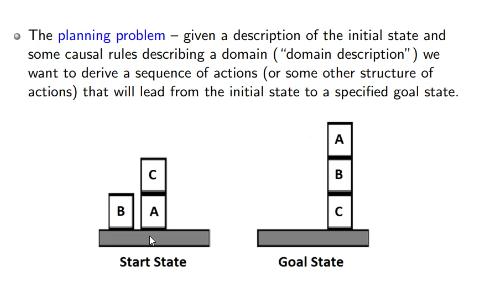
\includegraphics[width=200px]{../img/2022-03-26-23-59-10.png}
	      \end{align}
	\item Explanation problem - given some casual rules describing a domain, we want to discover facts about our given state
	      \textit{You wake up in the morning and you head downstairs in the kitchen theres a plate on the table and a bowl with a little milk left in, you can then say by assumption that your housemake was awoke before you and already had their breakfast}

\end{itemize}
\subsection{Terminology}
\begin{enumerate}
	\item \begin{definition}[Fluents]
		      Where the Truth varies over a period of time, think of them as a boolean state variable,
		      Like when a person x lies, but sometimes they can state the truth, it would follow that logic

		      we can also call this :
		      \textit{Temporal Propositional statements}
	      \end{definition}
	\item \begin{definition}[Time instances and time periods]
		      In short, year month day, or what happend on that date, we state to be time instances
		      for example
		      Last year my university decided to do in person exams to F every CS student over this allows us to give an initiation of our time  which leads into what occoured
	      \end{definition}
\end{enumerate}

We generate new fluences when a state is changed, for example in the image above, when you have your start state, b [c,[a]] in case you see that every variable there is in flux, whihch would imply that we would have to move c from a, and then move b to a etc ... to get to our goal state

\subsection{Frame problem}
The frame problem is about finding a great way to handle non change .
\begin{itemize}
	\item Peristence or Intertia - the assumption that the facts are not affect by its actions - such that they would hold the same truth value after the action, as they had before hadn

	\item The root of the problem lies in the fact of what the domain would represent

	\item  For smaller domains, with just a small number of fluents, and action types, we can just write it out properly.
\end{itemize}
To most AI researchers, the frame problem is the challenge of representing the effects of action in logic without having to represent explicitly a large number of intuitively obvious non-effects

types of problems
\begin{enumerate}
	\item Qualification problem - exhuastivly specifying preconditions of an action
	\item Computational fram to verify what was inferred

	\item Ramification problem - problem of exhastively specifying the effects of an action - think of chess


\end{enumerate}
TODO: Write more about Frame problem, as im not 100 \% sure how this works

\subsection{Situational Calculus}
The situation calculus is a logic formalism designed for representing and reasoning about dynamical domains. It was first introduced by John McCarthy in 1963. The main version of the situational calculus that is presented in this article is based on that introduced by Ray Reiter in 1991. Wikipedia
\textit{Domain - tend to be in first order logic :}\\
\begin{itemize}
	\item Fluents bassicly the item you are trying to change
	\item Actions the function you are pushing on those fluents
	\item Situations like an instance of the current state
\end{itemize}

\begin{align}
	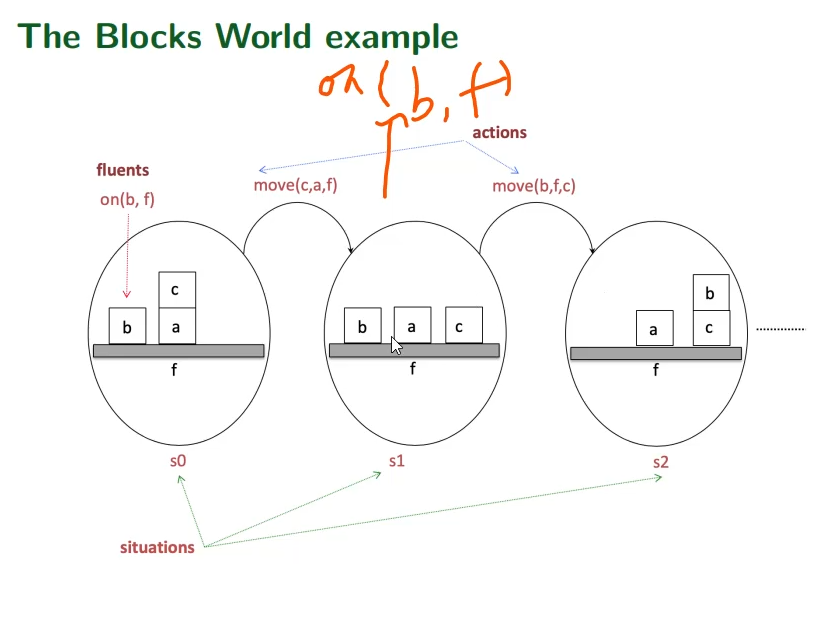
\includegraphics[width=200px]{../img/2022-03-27-00-44-10.png}
\end{align}
\begin{align}
	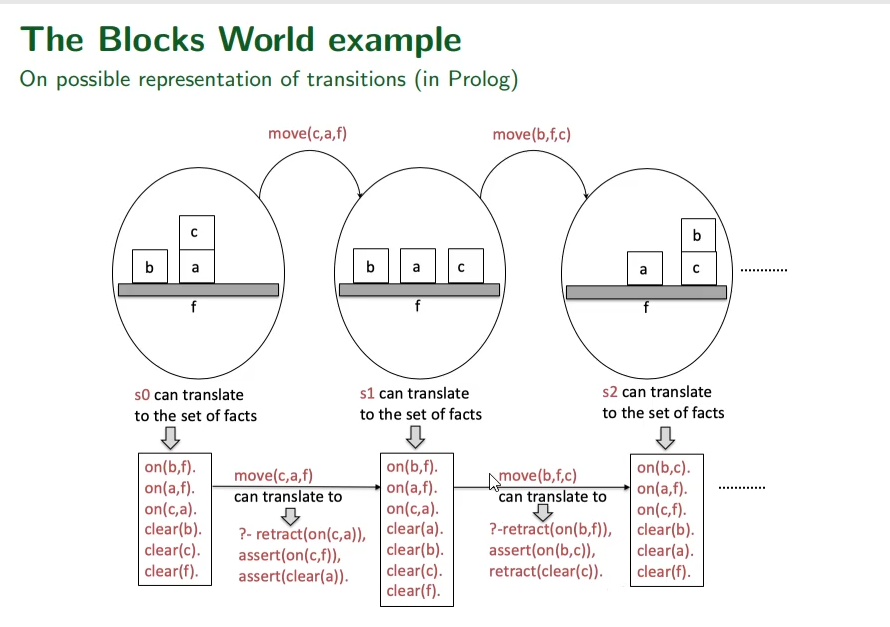
\includegraphics[width=200px]{../img/2022-03-27-00-46-27.png}
\end{align}

\begin{itemize}
	\item Remover and append operatiions within a fleucen
	\item Representation of actions as it stands does not check whether it is possible for a block to be moved from one place to another $\implies$ They dont check if something has been moved
	\item How can you improve cause and effect
\end{itemize}
\textit{Situation Calculus is trying to deal with the reasoning of the present }

We can use situational calculus to represent the current condition of a state.
\subsubsection{Situational Calc state Representation}
Situational Calc is defined through states

if you look at the image above we have multiple situations, from s1 to s3, with different fluents and actions that have been made upon some given variable
\begin{align}
	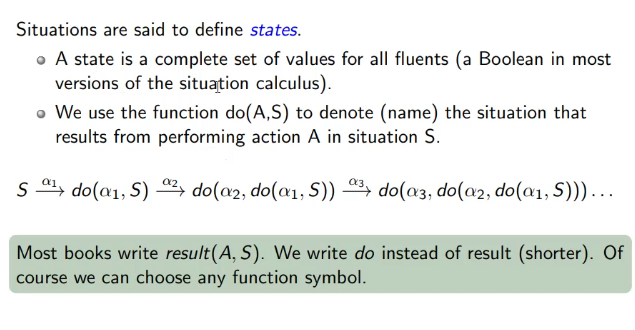
\includegraphics[width=200px]{../img/2022-03-27-02-05-12.png}
\end{align}

\subsubsection{Language}
\subsubsection{Axioms}
\subsubsection{Examples}
\subsection{Summary}

\end{document}
